\section{Results}

\subsection{Significant overlap of fungal communities of lung and gut contrary to bacteria}

Intersection analysis of bacterial and fungal communities between sputum and stool samples reveals increased overlap of fungal communities between the lung and gut, contrary to bacteria. Three bacterial genera including \emph{Lactobacillus, Prevotella} and \emph{Streptococcus} compared to six fungal genera including \emph{Candida, Cryptococcus, Curvularia, Debaryomyces, Lodderomyces} and \emph{Saccharomyces} were present in both sputum and stool samples. Interestingly, upon assessment of diversity between the sputum and stool samples, a similar pattern is observed. Overall, mycobiome exhibits a decreased diversity compared to microbiome. Further, an increased diversity of bacteria is found in the gut compared to the lung whereas the fungal diversity doesn't change. 

\begin{figure}[h]
	\centering
	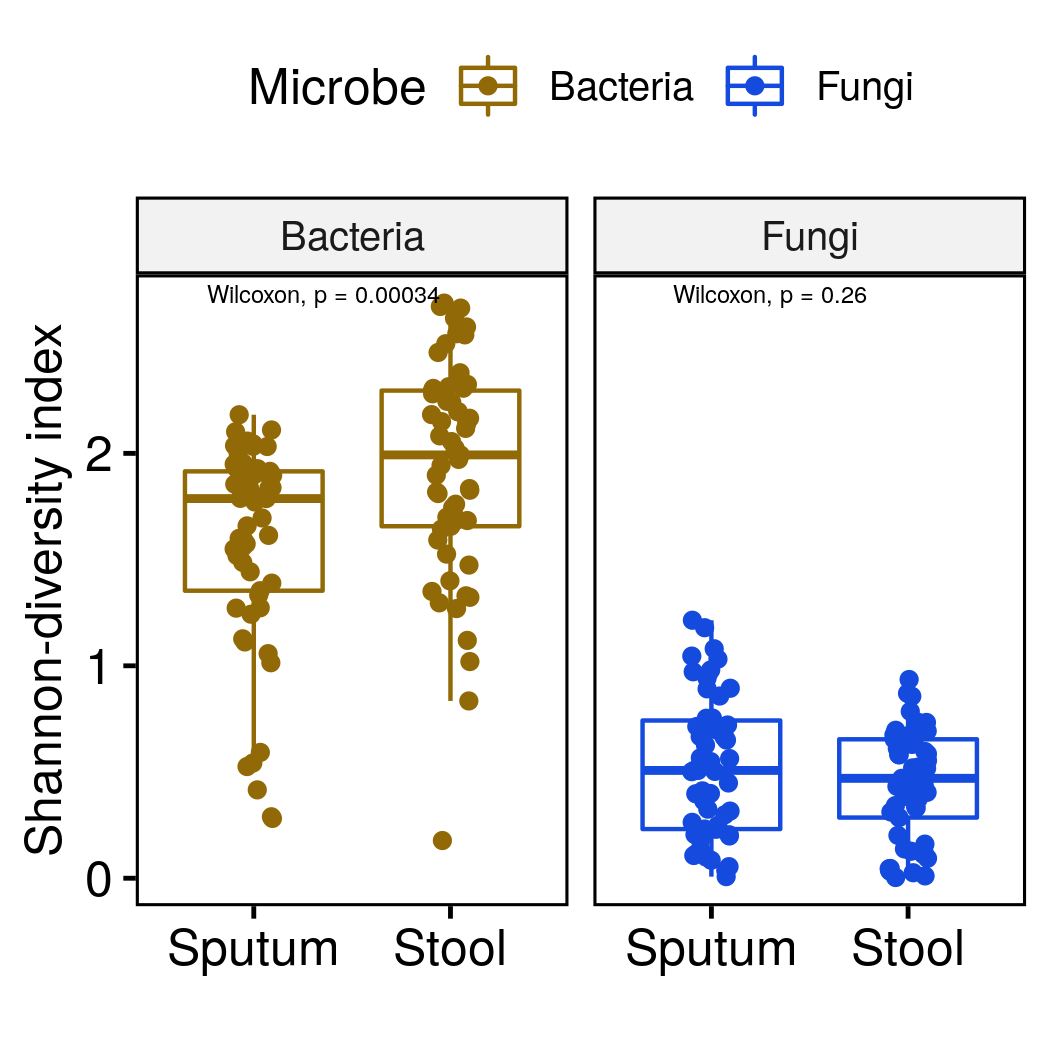
\includegraphics[width=0.5\textwidth]{image/diversity.png}
	\caption{A boxplot illustrating the difference in Shannon-diversity index of the Microbiome (Ochre) and Mycobiome (Blue) between the sputum (Lung) and stool (Gut) samples. Statistical significance of these differences were calculated using `wilcoxon test' and are indicated above as p-values.}
	\label{res2_fig1}
\end{figure}

\subsection{Co-occurrence analysis reveals lung – gut microbial (bacteria and fungi) interactions suggestive of a potential lung-gut axis.}


MOFA2 analysis reveals factors, highly contributed by the Gut bacteria and associated with exacerbations. 

Integrating microbiomes (bacteria and fungi) from lung and the gut, following clustering identifies patients with increased risk of exacerbation, Reiff score and FACED with no difference in lung function. 

High-risk patients exhibit significantly increased \emph{Candia} in Gut, \emph{Fusobacterium} in Lung, increased lung-gut microbial interaction (35\%>29\%) and movement of Streptococcus between lung and gut, illustrating a dysregulated lung-gut axis.